\documentclass[runningheads]{llncs}
\usepackage[utf8]{inputenc}
\usepackage{graphicx}
\usepackage{amsmath}
\usepackage{amsfonts}
\usepackage{amssymb}
\usepackage[caption = false]{subfig}
\usepackage[english,main=spanish]{babel}
% If possible, figure files should be included in EPS format.
%
% If you use the hyperref package, please uncomment the following line
% to display URLs in blue roman font according to Springer's eBook style:
% \renewcommand\UrlFont{\color{blue}\rmfamily}


\begin{document}
%
\title{Uso de información extraída de imágenes compartidas en Twitter para predicción de género en escenarios multilingüe}

%\titlerunning{Abbreviated paper title}
% If the paper title is too long for the running head, you can set
% an abbreviated paper title here

\author{First Author\inst{1}\orcidID{0000-1111-2222-3333} \and
Second Author\inst{2,3}\orcidID{1111-2222-3333-4444} \and
Third Author\inst{3}\orcidID{2222--3333-4444-5555}}
%
\authorrunning{F. Author et al.}
% First names are abbreviated in the running head.
% If there are more than two authors, 'et al.' is used.
%
\institute{Princeton University, Princeton NJ 08544, USA \and
Springer Heidelberg, Tiergartenstr. 17, 69121 Heidelberg, Germany
\email{lncs@springer.com}\\
\url{http://www.springer.com/gp/computer-science/lncs} \and
ABC Institute, Rupert-Karls-University Heidelberg, Heidelberg, Germany\\
\email{\{abc,lncs\}@uni-heidelberg.de}}

\maketitle

\begin{abstract}
The abstract should briefly summarize the contents of the paper in
150--250 words.

\keywords{First keyword  \and Second keyword \and Another keyword.}
\end{abstract}

\section{Introducción}

El contenido compartido en redes sociales incluye información 
en distintas modalidades como texto, imágenes, audio y video.
Toda estos datos pueden utilizarse para extraer información
valiosa de los usuarios. 
La tarea de perfilado de autores (AP por sus siglas en inglés), a través
del análisis de contenido compartido, busca determinar características demográficas 
específicas como género, edad, personalidad, legua nativa u orientación 
política \cite{rangel_rosso_montes-y-gomez_potthast_stein}. La identificación de tales 
aspectos puede aplicarse en una gran variedad de campos. Por ejemplo, la detección del 
género es útil en márketing y publicidad, donde las empresas pueden estar interesadas
en si le gustará o no un producto a un grupo demográfico \cite{miller_dickinson_hu_2012}.
También, dentro de la criminalística, es de interés detectar cuando alguien falsifica su género en internet \cite{cheng_chandramouli_subbalakshmi_2011}. 


Existen varias conferencias cuya meta 
es promover la investigación en áreas de recuperación
de información. Entre ellas están la Text REtrieval Conference (TREC) y la 
iniciativa CLEF (Conference and Labs of the Evaluation Forum, anteriormente 
conocida como Cross-Language Evaluation Forum). Dentro de esta última, se 
encuentra el PAN, una serie de eventos científicos y tareas sobre textos 
forenses y estilometría de textos digitales.
%  \cite{pan}. 

El objetivo de la tarea
de perfilado de autores del PAN 2018 fue abordar la identificación de género
desde una perspectiva multimodal donde además de texto se
incluyeron imágenes \cite{rangel_rosso_montes-y-gomez_potthast_stein}.
Para cumplir el propósito de la tarea, se brindó un conjunto de datos
obtenido de Twitter, el cual comprende tres idiomas: árabe, inglés y español.
La tarea permitía la clasificación para un subconjunto de idiomas; usando sólo texto, imágenes o haciendo una fusión de las dos fuentes de información.

A partir de los resultados obtenidos usando sólo imágenes 
 \cite{rangel_rosso_montes-y-gomez_potthast_stein}, se pudo observar que es posible 
utilizar información de éstas para el perfilado de usuarios.
La hipótesis de nuestro trabajo es que las imágenes de una colección para un
idioma  pueden ser útiles para identificar el perfil en otro idioma. 
Lo anterior es útil cuando no se cuenta con la cantidad suficiente de datos
para un grupo de usuarios en un idioma, pero sí para otros idiomas. Por ejemplo,
en la tarea de perfilado de autores del PAN, se cuentan con el doble de usuarios
en inglés y español en comparación a los del idioma árabe.

La principal contribución de nuestro trabajo es la confirmación
de que, para la tarea de identificación de género, las imágenes son independientes del 
idioma de los usuarios que las comparten. 

% A través de una extracción del contenido
% semántico de las imágenes de cada usuario podemos entrenar un modelo
% de manera eficiente y eficaz, para cada posible subconjunto de imágenes compartidas por los usuarios sean
% independientes del idioma permite utilizar
% un modelo, para clasificación de género, entrenado con imágenes de usuarios 
% en un idioma diferente al idioma de los usuarios sobre el que se desea aplicar.




% \begin{itemize}
%     \item Describir la tarea de perfilado de autores.
%     \item Predicción de género, ¿por qué? Marketing, otra motivación
%     sería mejor.
%     \item Uso de texto e imágenes para perfilado. Mencionar que 
%     utilizaré imágenes.
%     \item Hablar sobre los foros de evaluación, PAN 2018. Describir la
%     tarea.
%     \item Hablar de los resultados obtenidos por Takahashi y Ezra. El
%     trabajo del último sirve como base para mi proyecto.
%     \item Describir el problema de la clasificación de género 
%     usando imágenes de usuarios en otro idioma, ¿cómo la atacaré?,
%     ¿el idioma importa?, ¿es un problema el tamaño de los conjuntos de 
%     datos en un idioma?
%     \item Contribuciones.
% \end{itemize}
\section{Trabajo relacionado}

En la tarea del PAN 2018 los participantes identificaron el género
de usuarios de Twitter a través de una perspectiva multilingüe y multimodal. Los
datos provistos incluyen imágenes, tuits y cubren tres idiomas: árabe, inglés y
español. Los participantes utilizaron diferentes enfoques para resolver la tarea,
donde las soluciones predominantes aplicaron técnicas de aprendizaje profundo.
Los enfoques para la clasificación de imágenes se pueden agrupar en tres tipos:
\begin{enumerate}
    \item Basado en reconocimiento de rostros.
    \item Basados en modelos pre-entrenados y herramientas de procesamiento de
    imágenes como ImageNet.
    \item Características extraídas ``a mano'' como histogramas de color y bolsas 
    de palabras visuales.
\end{enumerate}

Respecto al segundo tipo de enfoque, los mejores resultados se obtuvieron 
con la extracción de características semánticas a partir de las 
imágenes \cite{rangel_rosso_montes-y-gomez_potthast_stein}.
Los mejores resultados para la clasificación usando imágenes los obtuvieron los
autores en \cite{takahashi_tahara_nagatan_miura_taniguchi_ohkuma}, quienes utilizaron 
un modelo pre-entrenado de red neuronal convolucional (CNN por sus siglas en inglés) 
basado en ImageNet. En algunos de los autores en los primeros puestos como \cite{aragon2018straightforward}, 
\cite{takahashi_tahara_nagatan_miura_taniguchi_ohkuma} y \cite{sierra_gonzales} utilizaron como modelo, para la extraccón de características, la red VGG16 \cite{zisserman_simonyan_2015}, donde \cite{sierra_gonzales} adicionalmente usó ResNet50 \cite{7780459} para comparar resultados, obteniendo mejores resultados con la última.

Nuestra propuesta sigue el mismo esquema que el de \cite{aragon2018straightforward}.
Donde utiliza el vector generado por la capa de salida. Este vector es una
distribución de probabilidad sobre mil categorías, compuestas por objetos y escenas
que puede contener la imagen. Como cada autor cuenta con diez tuits de imágenes,
se obtiene un vector promedio para representar a cada usuario y éste es utilizado sobre otro modelo para clasificar entre dos géneros: masculino y femenino. 
Los trabajos anteriores, sólo indican los resultados de la evaluación de los
modelos de clasificación con un enfoque monolingüe. Nuestra propuesta es desde
una perspectiva \textbf{¿croslingüe, crosslingüe?}.

% Ap-
% proaches based on face recognition do not belong to the best, which may be rooted inthe fact that many images do not show faces—and if, the contained faces do not depict
% the author.
% \begin{itemize}
%     \item Takahashi, Ezra.
%     \item Buscar qué se ha hecho en escenarios multilingüe.
%     \item Cross lingual pretraining.
%     \item GENDER PREDICTION BASED ON SEMANTIC ANALYSIS OF SOCIAL MEDIA 
%     IMAGES.
% \end{itemize}



\section{Solución propuesta}

Para poder mostrar que las imágenes compartidas son independientes
del idioma de los autores, nuestra propuesta consiste en entrenar clasificadores
con diferentes combinaciones de los conjuntos de imágenes de usuarios en los
tres idiomas. Después del entrenamiento de los posibles modelos, éstos se
prueban utilizando los conjuntos de los usuarios en cada idioma. Por ejemplo,
podemos entrenar un modelo de aprendizaje utilizando las imágenes de los
autores del idioma español y árabe. Posteriormente, evaluamos el desempeño
de ese modelo utilizando los conjuntos de imágenes de prueba de los usuarios
en español.

Nuestra solución se divide en dos partes; la obtención de un vector
de características que represente a cada usuario y el entrenamiento y 
prueba de los modelos. 

\subsection{Extracción de características semánticas de las imágenes}

Contamos con diez imágenes compartidas por cada usuario. La representación
de cada una de las imágenes se extrae a partir de un modelo de CNN
pre-entrenado, en nuestro trabajo utilizamos dos modelos VGG16 y ResNet50 para
comparar cuál tiene un mejor desempeño.
Cualquiera de los dos modelos genera un vector con una distribución 
de probabilidad sobre 1000 etiquetas posibles, estas etiquetas son objetos 
y escenas. Para obtener únicamente un vector de características que represente
a cada autor, promediamos los vectores de las diez imágenes. Los vectores
promedios serán los que se utilicen para el modelo de aprendizaje. En la Figura 
\ref{fig:img_representation} se muestra de manera gráfica lo descrito anteriormente.


\begin{figure}
    \centering
    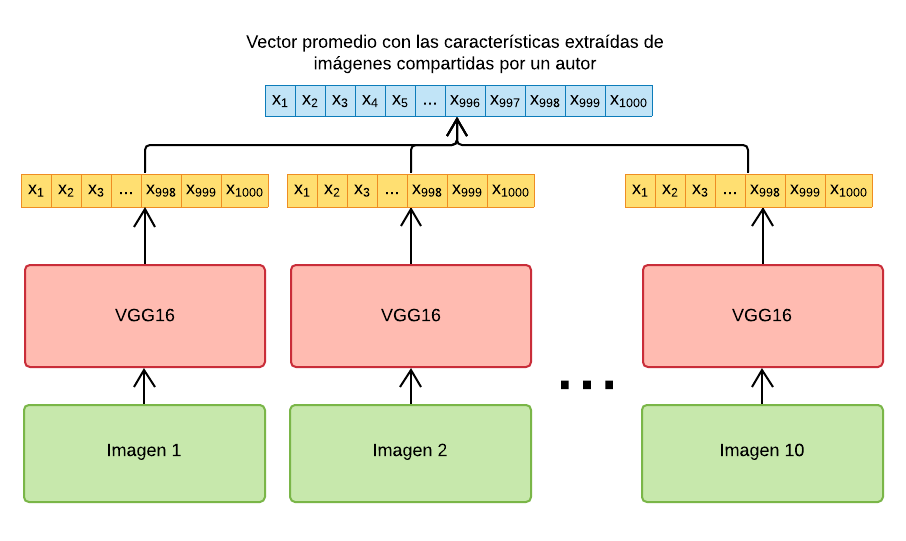
\includegraphics[scale=0.3]{img/features_extraction.png}
    \caption{Caption}
    \label{fig:img_representation}
\end{figure}


\subsection{Esquema de clasificación}

Construimos siete clasificadores para identificación del género de los autores, uno por 
cada subconjunto de las colecciones de imágenes de usuarios en los tres diferentes 
idiomas. Esto es, dado un conjunto $\mathbb{X} = \{\text{Árabe}, \text{Español}, \text{Inglés}\}$, donde cada elemento de $\mathbb{X}$ es una colección de 
representaciones de las imágenes de 
usuarios del respectivo idioma, el i-ésimo clasificador se entrenó con una colección 
$X_i \subseteq \mathbb{X}$ y $X_i \neq \varnothing$. Para este trabajo
el algoritmo de aprendizaje utilizado fue una máquina de vectores de soporte (SVM por 
sus siglas en inglés) con un kernel lineal. Después del entrenamiento 
de cada uno de los posibles clasificadores, éstos se evalúan con una colección $Y \in \mathbb{X}$. En la Figura \ref{fig:classifier} se muestra el esquema utilizado
para el entrenamiento y prueba de un clasificador.

\begin{figure}[!h]
    \centering
    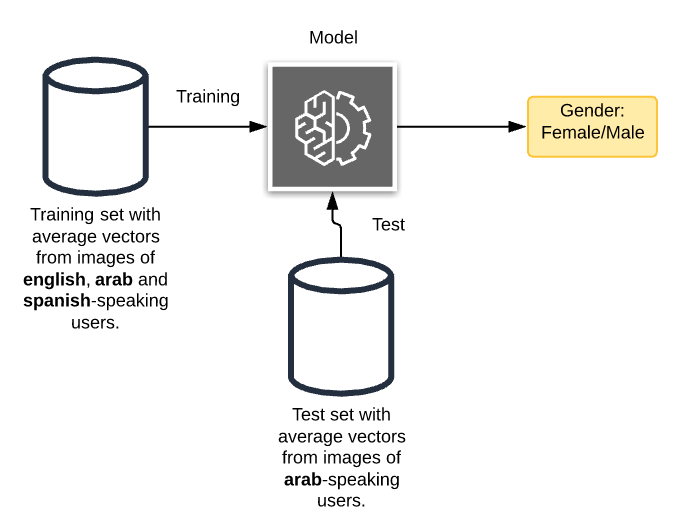
\includegraphics[scale=0.3]{img/classifier_scheme.png}
    \caption{Caption}
    \label{fig:classifier}
\end{figure}


\section{Experimentos}

La colección de imágenes es la de la tarea de perfilado de autores del PAN 2018
\cite{rangel_rosso_montes-y-gomez_potthast_stein}, donde se disponen de diez imágenes por cada autor y el número de autores de cada género es el mismo. El cuadro \ref{table-datasets}
muestra una descripción de los conjuntos de datos utilizados con respecto al número
de usuarios y al idioma de éstos.

La base para compararnos son las pruebas monolingües, es decir, aquellos
clasificadores entrenados y evaluados con imágenes de usuarios del mismo idioma.
Como los conjuntos de datos están balanceados con respecto al número de mujeres
y de hombres, la medida de evaluación para comparar los distintos clasificadores
es la exactitud, es decir, la proporción de muestras clasificadas correctamente.


Para la implementación empleamos las biblioteca de Python para aprendizaje 
profundo y aprendizaje automático Keras y scikit-learn, respectivamente. La primera
para extraer las representaciones de las imágenes de los usuarios con los modelos
pre-entrenados (VGG16 y ResNet50) y la segunda para construir y evaluar las SVM
para identificación de género. 
% Todo el software desarrollado está disponible en
% \url{https://github.com/ivanfeliciano/image-labeling-author-profiling}.

\begin{table}[]
\caption{Número de usuarios por cada idioma para los conjuntos de entrenamiento y de prueba.}\label{table-datasets}
\centering
\begin{tabular}{|l|l|l|l|l|}
\hline
              & Árabe & Español & Inglés & Total \\ \hline
Entrenamiento & 1500  & 3000    & 3000   & 7500  \\ \hline
Prueba        & 1000  & 2200    & 1900   & 5100  \\ \hline
Total         & 2500  & 4900    & 5200   & 12600 \\ \hline
\end{tabular}
\end{table}

\section{Resultados}


\subsection{Comparación de los enfoques monolingüe y crosslingüe}


\begin{table}
\centering
\begin{tabular}{|l|l|l|l|} 
\hline
Idioma entrenamiento & Idioma de prueba & Exactitud VGG16 & Exactitud ResNet50  \\ 
\hline
Árabe                & Inglés           & 0.6289473684    & 0.6363157895        \\ 
\cline{2-4}
                     & Español          & 0.625           & 0.6168181818        \\ 
\cline{2-4}
                     & Árabe            & 0.676           & 0.684               \\ 
\hline
Español              & Inglés           & 0.6747368421    & 0.6521052632        \\ 
\cline{2-4}
                     & Español          & 0.6740909091    & 0.6468181818        \\ 
\cline{2-4}
                     & Árabe            & 0.696           & 0.683               \\ 
\hline
Inglés               & Inglés           & 0.6989473684    & \textbf{0.7010526316}        \\ 
\cline{2-4}
                     & Español          & 0.6668181818    & 0.6713636364        \\ 
\cline{2-4}
                     & Árabe            & 0.69            & 0.674               \\ 
\hline
Árabe Español        & Inglés           & 0.6763157895    & 0.6710526316        \\ 
\cline{2-4}
                     & Español          & 0.6659090909    & 0.6622727273        \\ 
\cline{2-4}
                     & Árabe            & \textbf{0.707}          & 0.698               \\ 
\hline
Árabe Inglés         & Inglés           & 0.6847368421    & 0.6978947368        \\ 
\cline{2-4}
                     & Español          & 0.6586363636    & 0.6659090909        \\ 
\cline{2-4}
                     & Árabe            & 0.694           & 0.699               \\ 
\hline
Español Inglés       & Inglés           & 0.6978947368    & 0.6989473684        \\ 
\cline{2-4}
                     & Español          & 0.675           & 0.6713636364        \\ 
\cline{2-4}
                     & Árabe            & 0.703           & 0.699               \\ 
\hline
Árabe Español Inglés & Inglés           & \textbf{0.7}             & 0.6978947368        \\ 
\cline{2-4}
                     & Español          & \textbf{0.6759090909}    & \textbf{0.6736363636}        \\ 
\cline{2-4}
                     & Árabe            & \textbf{0.707}           & \textbf{0.71}                \\
\hline
\end{tabular}
\end{table}


\subsection{Gráficas de las sumas de vectores de los hombres y mujers VGG16}

\begin{figure}
\subfloat{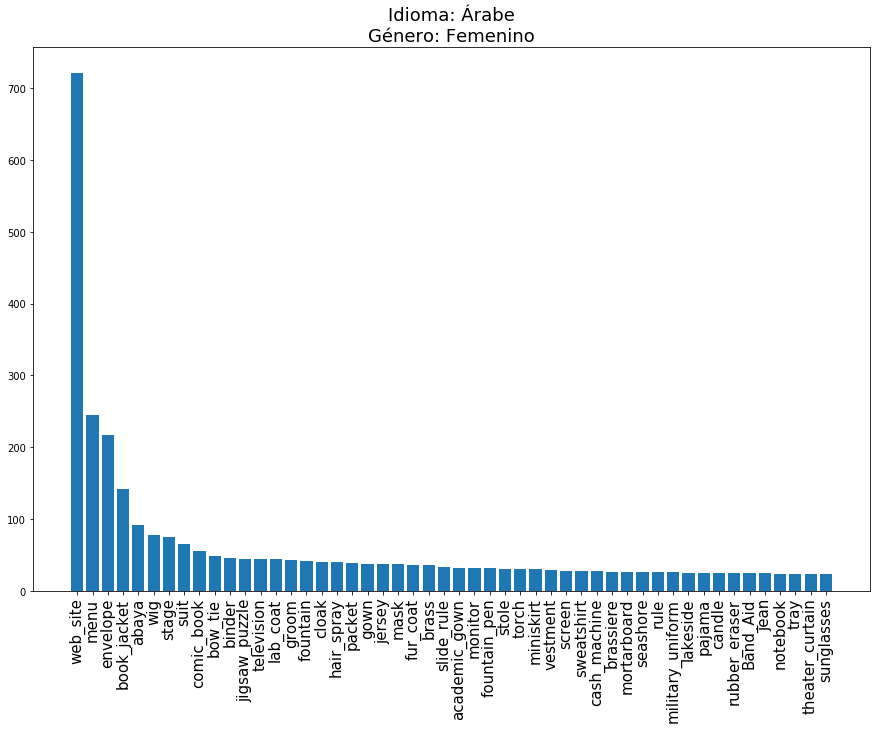
\includegraphics[width = 3in]{img/vgg16/AR_f.png}} 
\subfloat{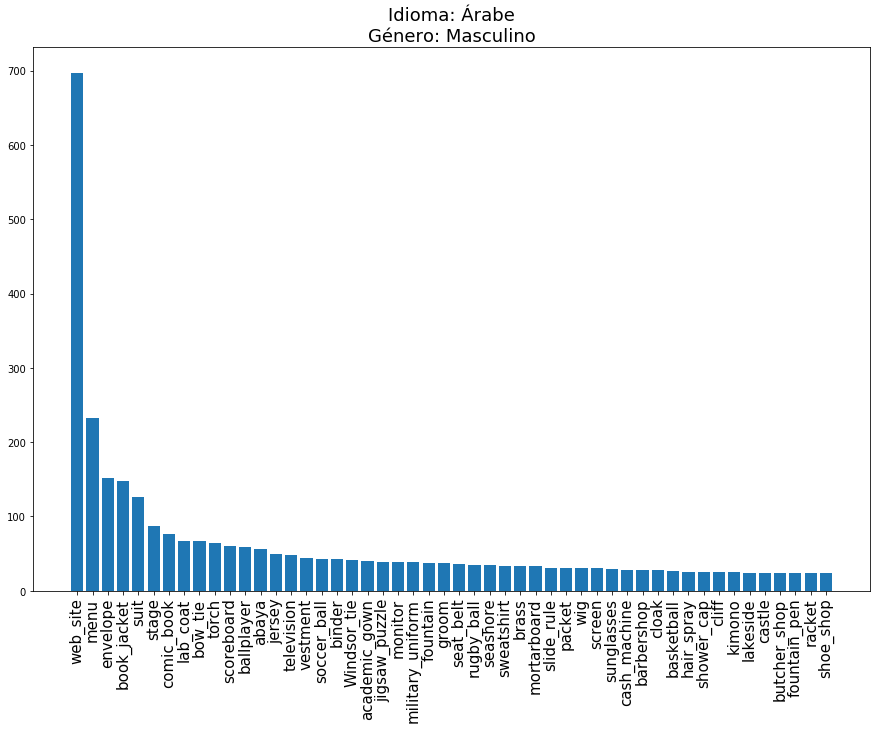
\includegraphics[width = 3in]{img/vgg16/AR_m.png}}\\
\subfloat{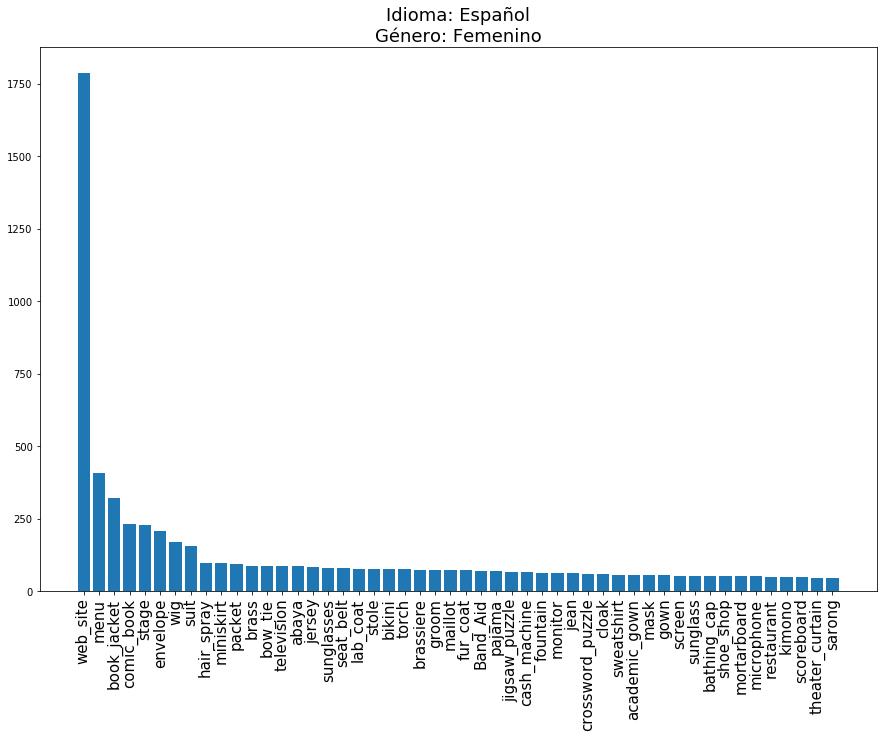
\includegraphics[width = 3in]{img/vgg16/ES_f.png}}
\subfloat{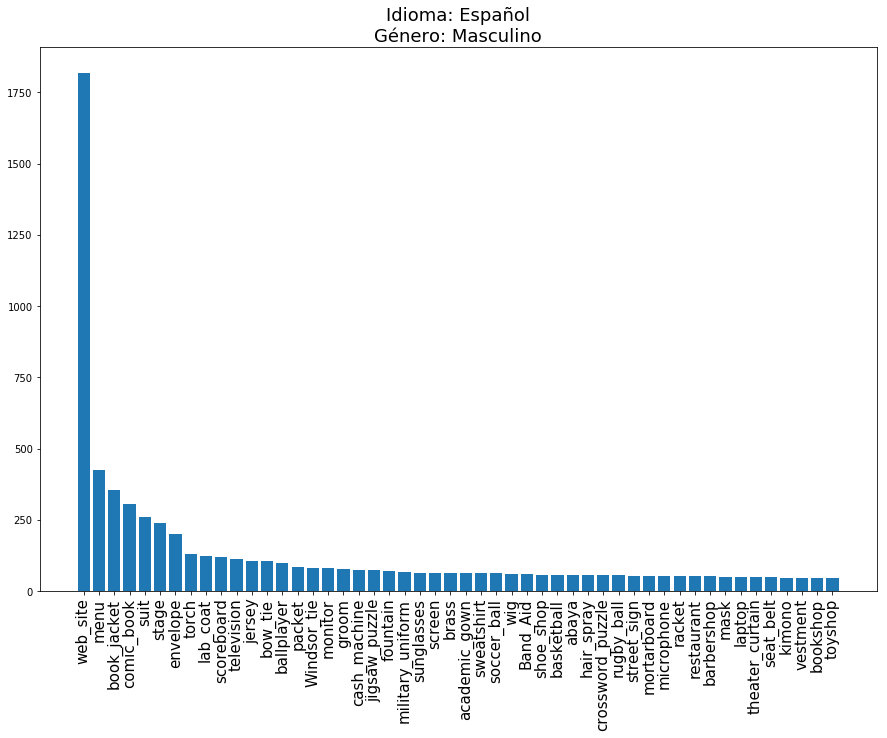
\includegraphics[width = 3in]{img/vgg16/ES_m.png}}\\ 
\subfloat{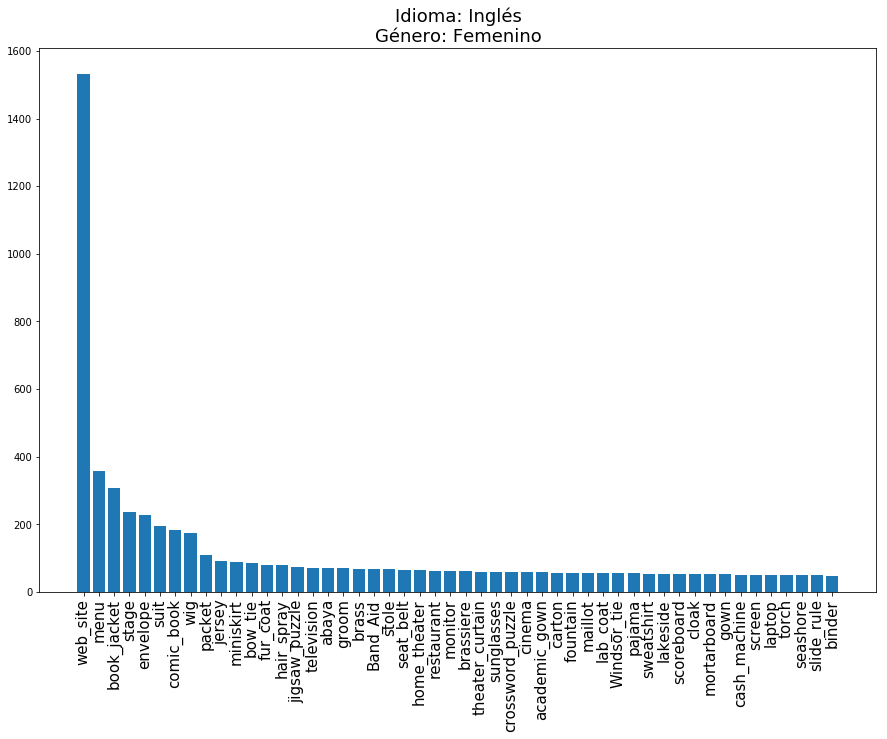
\includegraphics[width = 3in]{img/vgg16/EN_f.png}}
\subfloat{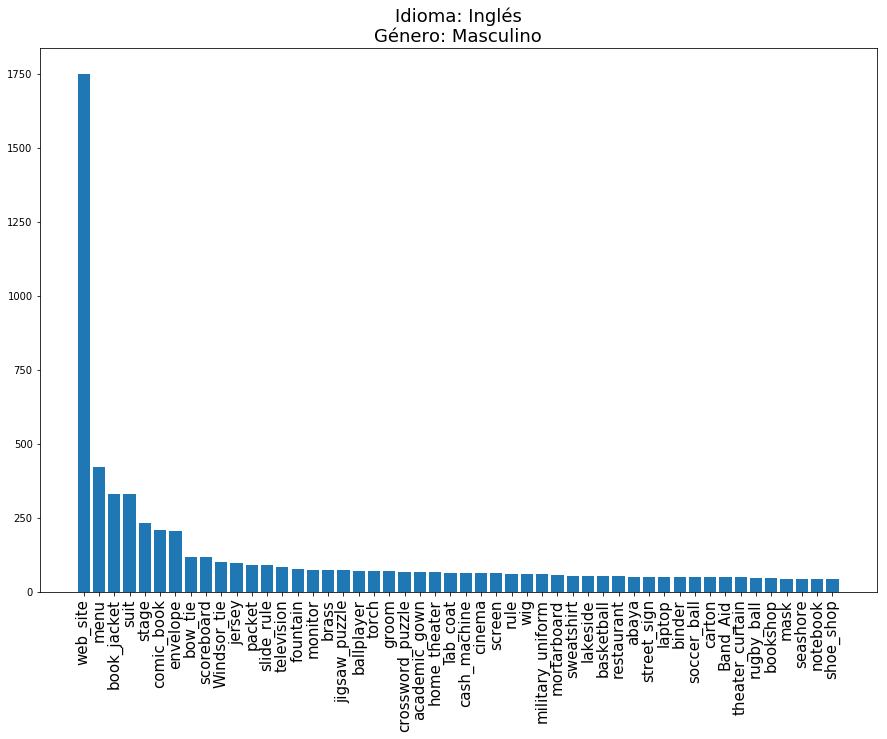
\includegraphics[width = 3in]{img/vgg16/EN_m.png}}
\caption{Caption}
\label{img-vgg16-freqs}
\end{figure}

\subsection{Gráficas de las sumas de vectores de los hombres y mujers Resnet50}

\begin{figure}
\subfloat{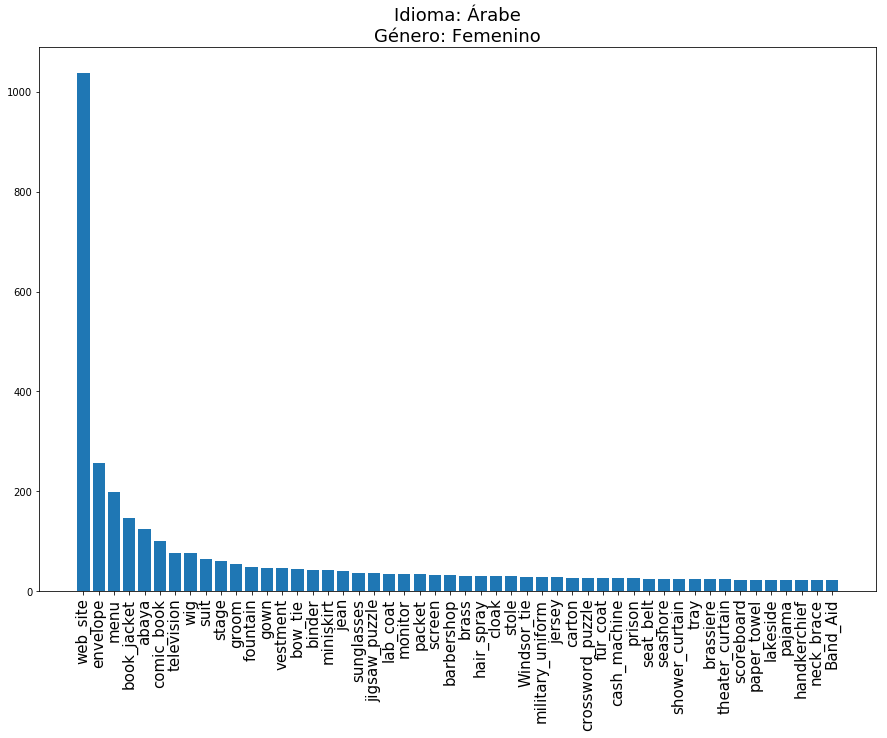
\includegraphics[width = 3in]{img/resnet/AR_f.png}} 
\subfloat{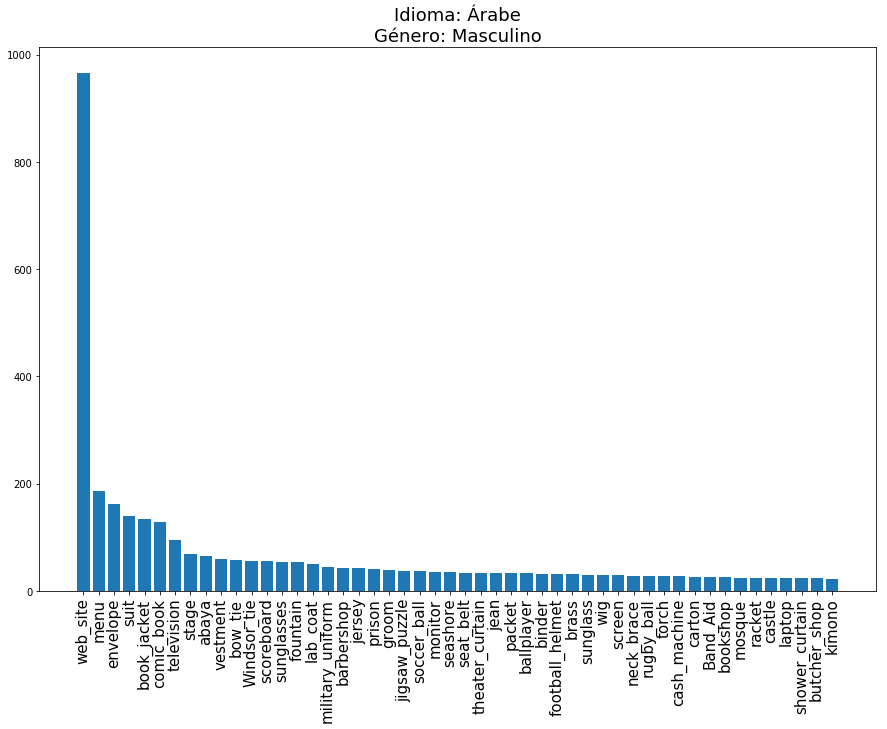
\includegraphics[width = 3in]{img/resnet/AR_m.png}}\\
\subfloat{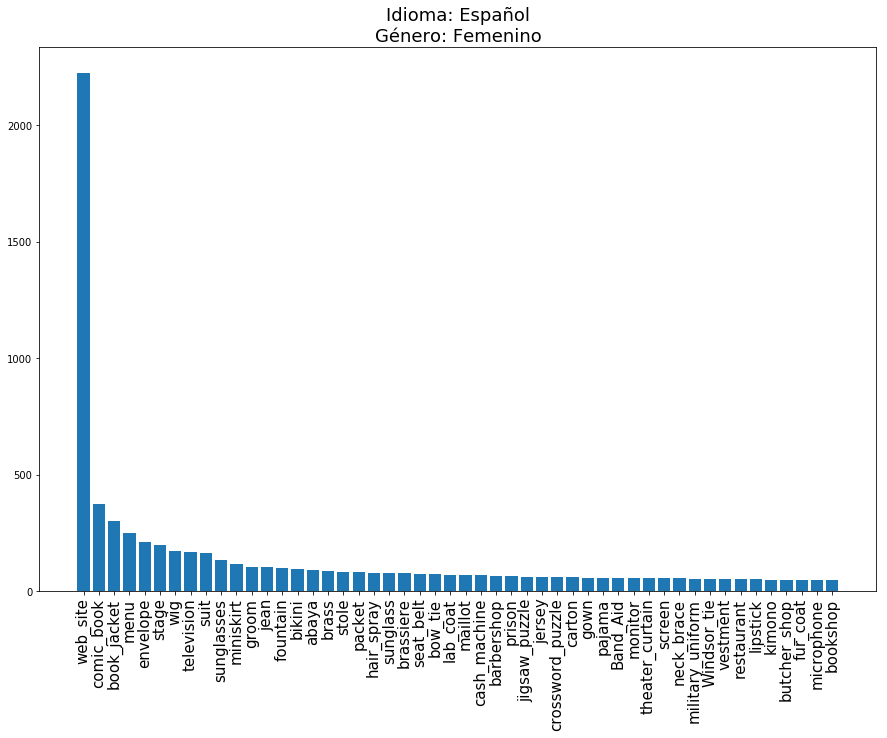
\includegraphics[width = 3in]{img/resnet/ES_f.png}}
\subfloat{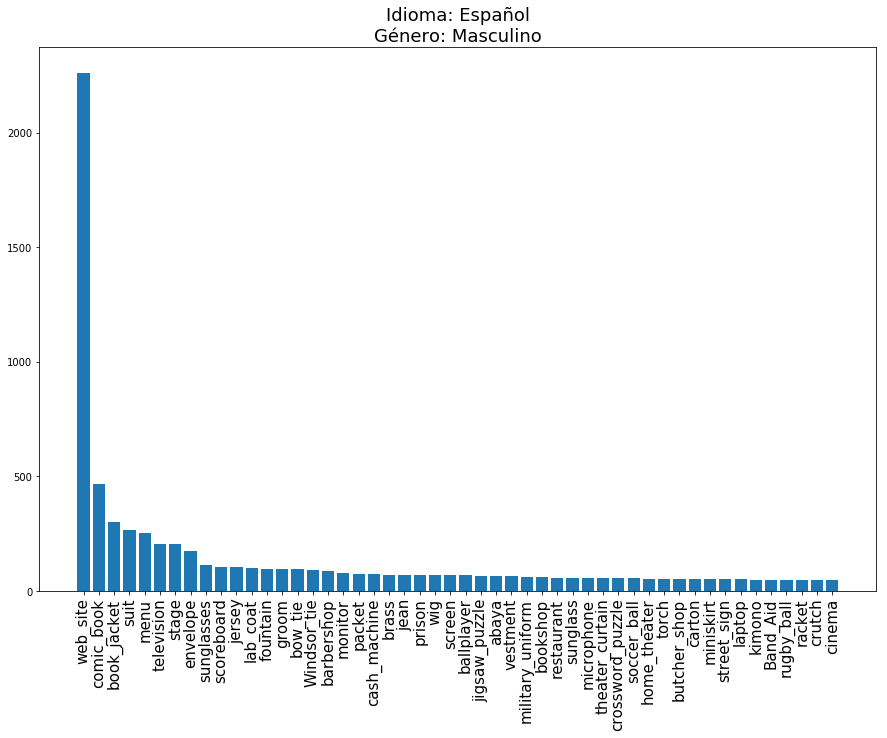
\includegraphics[width = 3in]{img/resnet/ES_m.png}}\\ 
\subfloat{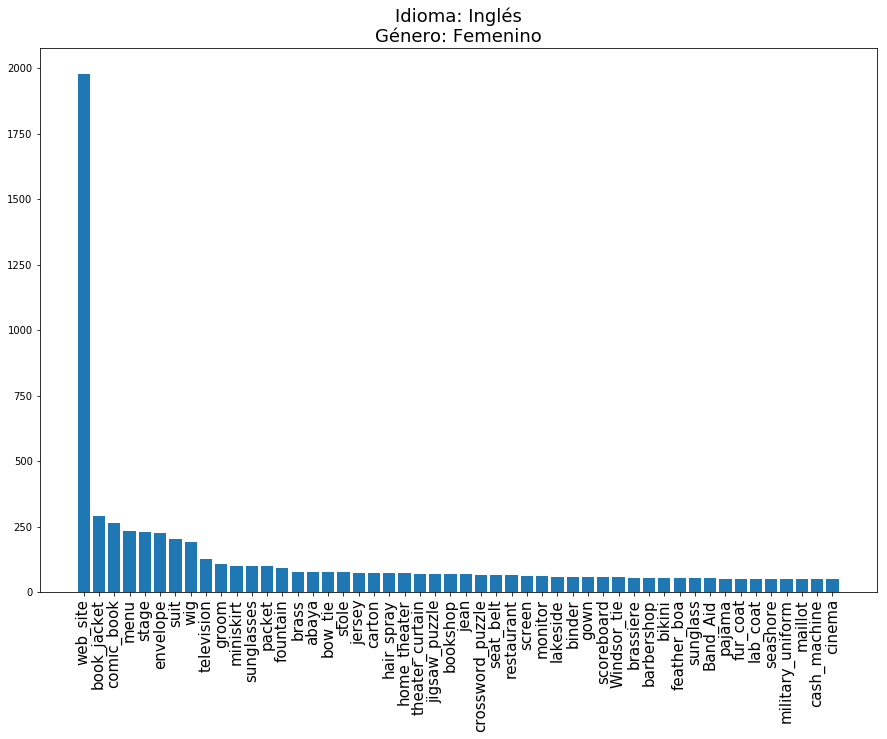
\includegraphics[width = 3in]{img/resnet/EN_f.png}}
\subfloat{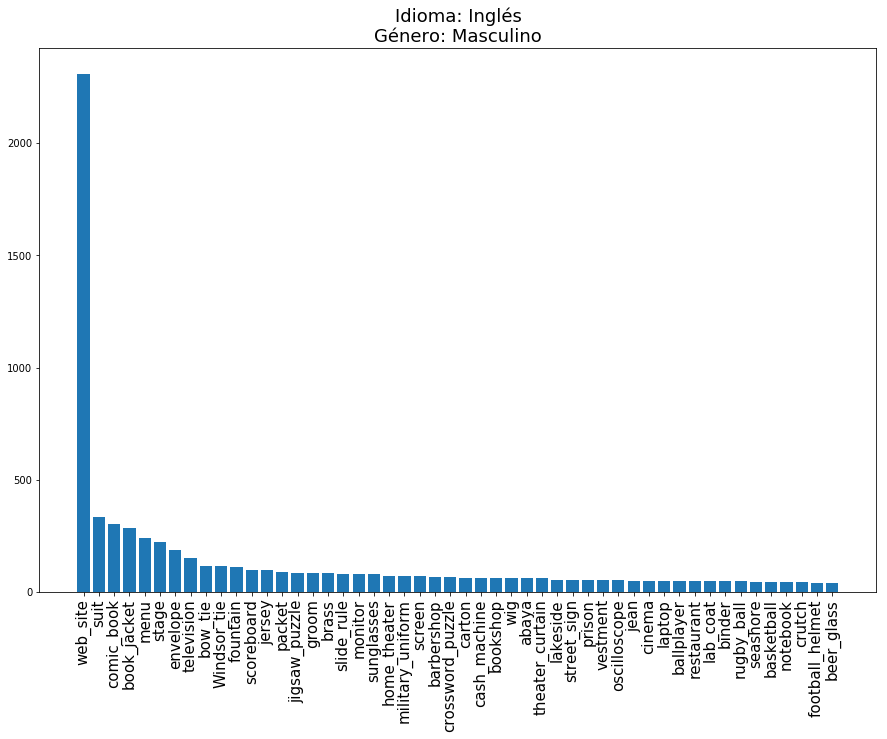
\includegraphics[width = 3in]{img/resnet/EN_m.png}}
\caption{Caption}
\label{img-resnet-freqs}
\end{figure}




\subsection{Tablas de correlación entre géneros e idiomas VGG16}
\begin{table}[]

\centering
\caption{Hombres vs. Hombres}
\label{male-vs-male-correlation}
\begin{tabular}{|l|l|l|l|}
\hline
        & Árabe        & Español      & Inglés       \\ \hline
Árabe   & 1            & 0.9821367303 & 0.9821702278 \\ \hline
Español & 0.9821367303 & 1            & 0.9946005346 \\ \hline
Inglés  & 0.9821702278 & 0.9946005346 & 1            \\ \hline
\end{tabular}
\end{table}

\begin{table}[]
\centering
\caption{Mujeres vs. Mujeres}
\label{female-vs-female-correlation}
\begin{tabular}{|l|l|l|l|}
\hline
        & Árabe        & Español      & Inglés       \\ \hline
Árabe   & 1            & 0.9711885725 & 0.9765954799 \\ \hline
Español & 0.9711885725 & 1            & 0.995615316  \\ \hline
Inglés  & 0.9765954799 & 0.995615316  & 1            \\ \hline
\end{tabular}
\end{table}


\begin{table}[]
\centering
\caption{Hombres (fila) vs Mujeres (columnas)}
\label{male-female-correlation}
\begin{tabular}{|l|l|l|l|}
\hline
        & Árabe        & Español      & Inglés       \\ \hline
Árabe   & 0.9798501212 & 0.9711885725 & 0.974166434  \\ \hline
Español & 0.9615626915 & 0.9894368692 & 0.9864575353 \\ \hline
Inglés  & 0.9633847896 & 0.9851604739 & 0.9877626583 \\ \hline
\end{tabular}
\end{table}


% \begin{itemize}
%     \item Análisis de resultados.
%     \item Tablas de las combinaciones que se probaron.
%     \item Selección de características.
%     \item Histogramas de ``frecuencias''.
%     \item Correlación entre los vectores de los hombres y mujeres
%     entre los idiomas.
% \end{itemize}


\section{Conclusiones y trabajo futuro}

\begin{itemize}
    \item ¿El idioma importa? 
    \item ¿Comparten lo mismo los usuarios del género $X$ en el idioma
    $Y$ y los usuarios del género $X$ en el idioma $\hat{Y}$.
    \item ¿Es suficiente el vocabulario con el que cuenta imagenet
    (1000 objetos y escenarios)?
    \item Extender el trabajo usando el enfoque no supervisado.
    \item Vocabulario abierto.
    \item Agrupamiento dentro de cada género.
\end{itemize}

\bibliographystyle{splncs04}
\bibliography{references}

\end{document}
